\documentclass{article}
\usepackage[utf8]{inputenc} %accenti
\usepackage{imakeidx}
\makeindex
\usepackage{graphicx}
\graphicspath{ {./images/} }
\usepackage{float}
\usepackage{amsmath}
\usepackage[colorlinks, linkcolor=blue]{hyperref}
\usepackage[italian]{babel}
\usepackage[backend=biber]{biblatex}
\usepackage[autostyle,italian=guillemets]{csquotes}
\addbibresource{sample.bib}
\usepackage{booktabs}
\usepackage[left = 3.8 cm, right = 3.8 cm]{geometry}
\usepackage{fourier} 
\usepackage{array}
\usepackage{makecell}
\title{\huge Percussion Drilling}
\author{ \large Onofrio Davide Caputo \\ \large Giuseppe Giorgio  \\ \large Francesco Pio Merafina}
\date{ \small Data esperimento: 6 Maggio 2022 \\ Data relazione: 10 Maggio 2022}

\begin{document}
\begin{figure}[t]
\hspace*{-2cm}
    
\includegraphics{Uniba.png}
\end{figure} 
\maketitle

\noindent \textbf{\Large Abstract}\\

\noindent L'esperienza realizzata consiste nell'utilizzo della tecnica del percussion drilling nella sue due varianti: mediante un treno di impulsi o mediante treni di burst di impulsi.
L'obiettivo è capire quale dei due metodi è il più adatto ad una foratura, in base all'analisi dei risultati ottenuti. 

\tableofcontents

\normalsize
\setlength{\columnsep}{20pt}
\twocolumn
\section{Introduzione}
Tra le tante lavorazioni laser, la foratura è certamente una delle più diffuse. Nell'esperienza si è fatto uso della tecnica del multi-pulse percussion, cioè una lamina di acciaio è stata perforata con un treno di impulsi. 

La particolarità dell'esperimento risiede nell'utilizzo di un generatore di burst, cioè uno strumento ottico che permette di creare da un singolo impulso un treno di sotto-impulsi. Tali sotto impulsi hanno la particolarità di essere distanziati pochissimo temporalmente. Per dare un ordine di grandezza, mentre gli impulsi iniziali distano temporalmente qualche $\mu s$, gli impulsi del burst distano solo qualche $ps$, ossia ben 6 ordini di grandezza in meno.
 É importante notare che il laser non è stato utilizzato per vaporizzare il materiale, ma per scioglierlo strato dopo strato. A causa di questo, si ottiene che il foro di entrata è diverso da quello di uscita. Infatti più il fascio laser entra in profondità, più materiale fuso viene espulso usando getti di vapore, compromettendo la qualità del foro e mettendo a rischio l'ottica del laser. 
 Si osserva anche il fenomeno del taper, ossia la riduzione della potenza del laser man mano che il fascio va in profondità, si può valutare mediante la seguente equazione:

\begin{equation}
    \theta=arctan(\frac{2h}{D_{in}-D_{out}})
\end{equation}

\begin{figure}[h!]
    \centering
    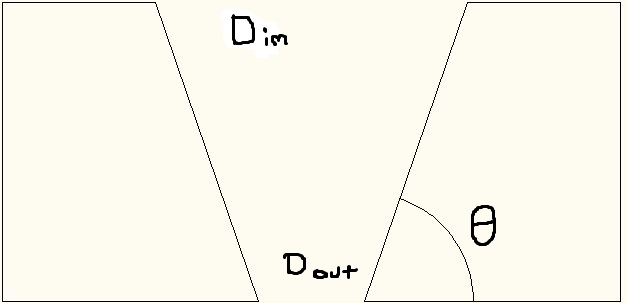
\includegraphics[width=\linewidth]{taper.jpg}
    \caption{Schematizzazzione del taper}
    \label{fig:taper}
\end{figure}
Lo scopo del nostro esperimento, è dunque osservare le differenza di tempo della foratura nelle diverse configurazioni e la diversa qualità dei fori ottenuti.
~
\section{Descrizione dell'apparato sperimentale}
La strumentazione usata consiste in una sorgente laser di $\lambda=1030nm$ con una frequenza di ripetizione di $200kHz$ ed un tempo d'impulso di $200fs$. La sorgente laser è stata utilizzata insieme ad una catena ottica lungo la quale abbiamo inserito il nostro generatore di burst. Esso consiste in 5 cristalli birifrangenti posti nel loro supporto ottico. Il fascio viene deviato su un portacampione munito di vite micrometrica. Tale vite è utile a muovere il campione, ossia una lamina di acciaio. Per poter misurare il tempo di foratura usiamo due fotocellule. La prima è posta di fianco al fascio, mentre la seconda è sotto il campione. Si misura la differenza temporale tra i segnali provenienti dai due fotodiodi osservando il segnale sullo schermo dell'oscilloscopio.
In realtà l'oscilloscopio riceve un terzo segnale, proveniente direttamente dal laser. Questo viene chiamato TRIGGER e di fatto è indistinguibile da quello del primo fotodiodo a causa di un'insufficiente risoluzione dell'elettronica.

Infine per poter osservare e misurare i fori abbiamo usato un microscopio elettronico insieme ad un software.

\section{Descrizione dell'esperimento}
Per poter realizzare la configurazione "a burst" è necessario aggiustare la strumentazione ottica consistente di cinque lamine birifrangenti in calcite.
Il principio di fondo è che se un fascio polarizzato verticalmente incide su un cristallo birifrangente con asse ottico a 45° rispetto alla sua polarizzazione, vengono creati due impulsi. Il primo è polarizzato nella direzione dell'asse ordinario e il secondo è polarizzato ortogonalmente ad esso.
Tra i due fasci ci sarà uno sfasamento temporale. 
Aggiustando l'orientazione dei cristalli si sono create tre (più una) configurazioni che sono elencate e spiegate di seguito.

\textbf{Prima configurazione:\\}
Contiene 32 burst ritardati l'uno dall'altro di $1.5ps$, realizzata disponendo gli assi ottici dei cristalli a 45° l'uno rispetto all'altro.

\textbf{Seconda configurazione:\\}
Contiene 2 burst ritardati l'uno dall'altro di $1.5ps$, realizzata disponendo gli assi ottici dei primi 4 cristalli paralleli all'impulso iniziale e l'ultimo a 45°.

\textbf{Terza configurazione:\\}
Contiene 2 burst ritardati l'uno dall'altro di $46.5ps$, realizzata mettendo il primo cristallo a 45° rispetto al fascio iniziale e tutti gli altri ad esso paralleli. 

\textbf{Quarta configurazione:\\}
É la configurazione no burst. 
\\
Per ogni configurazione si è esplorato mediante 5 potenze nominali diverse, rispettivamente di 170mW, 220mW, 270mW, 370mW e 520mW.
Per ogni potenza sono stati realizzati 5 fori e i tempi di foratura sono stati collezionati mediante una misura con l'oscilloscopio, come spiegato in precendenza.


\section{Analisi dei dati}
Raccolti i dati, questi sono stati successivamente analizzati sfruttando le funzionalità del software \textit{Microsoft Excel}.
\begin{figure}[h!]
    \centering
    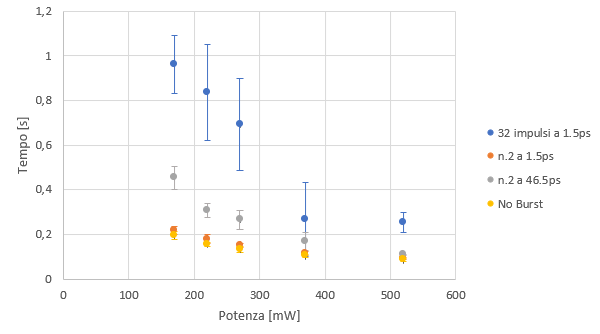
\includegraphics[width=\linewidth]{grafico-foratura.png}
    \caption{Gragico dei tempi di foratura in funzione della potenza fornita e del tipo di configurazione utilizzata}
    \label{fig:Grafico_foratura}
\end{figure}
Da un'analisi preliminare del grafico ottenuto, è facile notare le seguenti caratteristiche dell'andamento del tempo di foratura:
\begin{itemize}
    \item Il tempo di foratura diminuisce all’aumentare della potenza incidente;
    \item Il tempo di foratura diminuisce al diminuire del numero di sotto impulsi;
    \item A parità del numero di sottoimpulsi il tempo di foratura è minore quando tra i primi intercorre un tempo minore;
\end{itemize}

Ulteriore caratteristica del fenomeno in questione potrebbe essere derivata prestando attenzione alle differenze temporali relative per configurazioni differenti alla stessa potenza. In particolare è possibile notare che all'aumentare della potenza, i tempi di foratura di tutte le configurazioni tendono a compattarsi entro un determinato intervallo di tempo, vale a dire:
\begin{itemize}
    \item Per una potenza di $170 mW$ tutte le configurazioni agiscono entro un intervallo temporare di $0.77 ms$;
    \item Per una potenza di $270 mW$ tutte le configurazioni agiscono entro un intervallo temporale di $0.59 ms$;
    \item Per una potenza di $520 mW$ tutte le configurazioni agiscono entro un intervallo temporale di $0.17 ms$;
\end{itemize}
Questo comportamento osservato potrebbe indurre a pensare che per determinati valori di potenza fornita non ci sia più alcuna differenza apprezzabile tra le varie configurazioni.
Purtroppo questa conclusione è solo preliminare e avrebbe bisogno di ulteriori analisi per poter essere corroborata.

In un processo di lavorazione laser, come quello analizzato in questa esperienza, un altro fattore importante è la riproducibilità della lavorazione eseguita. Abbiamo associato questo parametro alla valutazione della deviazione standard associata ai tempi di foratura misurati, in particolare se la deviazione standard dovesse risultare contenuta, questa verrebbe associata ad una migliore riproducibilità della lavorazione, viceversa se la deviazione standard dovesse assumere valori troppo elevati, la lavorazione eseguita verrebbe ritenuta poco riproducibile.
\begin{figure}[h!]
    \centering
    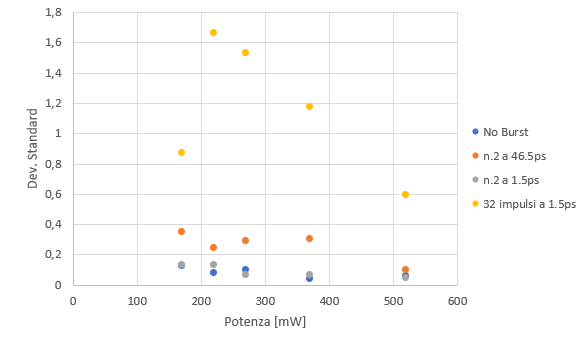
\includegraphics[width=\linewidth]{grafico-devstandard.foratura.png}
    \caption{Grafico della deviazione standard sui tempi misurati in funzione delle potenze fornite}
    \label{fig:dev_standard}
\end{figure}
Dall'analisi della figura riportata di sopra è possibile effettuare delle considerazioni riguardanti la riproducibilità delle lavorazioni effettuate, in particolare:
\begin{itemize}
    \item La riproducibilità è funzione del numero d'impulsi
    \begin{itemize}
        \item A basse potenze la riproducibilità aumenta al diminuire del numero di sottoimpulsi, in particolare la configurazione "No Burst" sarà la più riproducibile;
        \item Il maggior ritardo temporale implica una minore riproducibilità associata alle diverse configurazioni;
    \end{itemize}
    \item A potenze maggiori l'andamento varia, ad esempio nel caso di potenza a $520 mW$ osserviamo che:
    \begin{itemize}
        \item la configurazione a 32 impulsi risulta essere ancora la meno riproducibile;
        \item il ritardo temporale tra i sottoimpulsi causa ancora una diminuzione della riproducibilità della lavorazione;
        \item la configurazione "No Burst" e la configurazione a 2 impulsi con ritardo temporale di $1,5 ps$ sono le più riproducibili, ed in particolare la seconda risulta essere di poco la più riproducibile.
    \end{itemize}
\end{itemize}
Infine un ultimo parametro da tenere in considerazione al fine di valutare la qualità della lavorazione di foratura laser è l'angolo del taper, associato all'analogo fenomeno.
I dati riguardanti quest'ultima valutazione sono stati raccolti al microscopio elettronico, valutando il diametro d'ingresso e di uscita per i fori creati alla potenza di $520 mW$.
\begin{table}[h!]
\begin{center}
    \begin{tabular}{ | c | c | c | c|}
      \hline
      \thead{n=32 \\a 1,5ps} & \thead{n=2 \\ a 1,5ps} & \thead{n=2 \\a 46,5ps} & \thead{No \\burst} \\
      \hline
       $70,97^\circ$ &  \makecell{$72,52^\circ$}  & $79,52^\circ$  & $81,47^\circ$ \\
      \hline
    \end{tabular}
  \end{center}
 
    \caption{Tabella rappresentativa degli angoli del taper alla potenza di $520 mW$}
    \label{tab:tabella_angoli_taper}
\end{table}

\noindent In particolare questa tabella ci mostra in che modo al variare delle differenti configurazioni abbiamo una conseguente variazione dell'angolo di taper e quindi della qualità della foratura. In particolare al crescere dell'angolo di taper, la foratura avrà una qualità maggiore, ed è quello che accade al diminuire del numero di sottoimpulsi nella configurazione, rendendo la "No Burst" la più adatta ad effettuare operazioni di foratura con maggiore qualità di realizzazione.

\section{Conclusioni}
In conclusione, i risultati dell'esperimento mostrano chiaramente come la maggior riproducibilità del foro non si ottiene solo aumentando la potenza, ma anche diminuendo il numero di sottoimpulsi, il che ci porta ad affermare che la configurazione No burst sia la più indicata. 




\end{document}
